\documentclass[11pt]{article}

\usepackage[margin=1in]{geometry}
\usepackage{amsmath,amssymb,amsthm}
\usepackage{tikz}
\usetikzlibrary{calc,arrows.meta,decorations.pathreplacing,positioning,shapes.geometric}
\usepackage{graphicx}
\usepackage[expansion=false]{microtype}
\usepackage{xcolor}
\usepackage{hyperref}

\hypersetup{
  colorlinks=true,
  linkcolor=blue!50!black,
  citecolor=blue!50!black,
  urlcolor=blue!50!black
}

\newtheorem{theorem}{Theorem}
\newtheorem{proposition}[theorem]{Proposition}
\newtheorem{lemma}[theorem]{Lemma}
\newtheorem{corollary}[theorem]{Corollary}
\theoremstyle{definition}
\newtheorem{definition}[theorem]{Definition}
\newtheorem*{remark}{Remark}

\newcommand{\X}{X}
\newcommand{\Tr}{\mathrm{Tr}}

\title{Geometric Picture: Hidden Zeros, Chord Birth, and Why Locality Has to Hold\thanks{Section draft, intended as \S2 of the rewritten \emph{Locality and Unitarity of $\Tr(\phi^3)$ Tree Amplitudes from Hidden Zeros}.}}
\date{April 2026}

\begin{document}
\maketitle

\section*{Section 2 --- Geometric Picture}
\setcounter{section}{2}
\renewcommand{\thesection}{\arabic{section}}
\renewcommand{\thesubsection}{\thesection.\arabic{subsection}}

\noindent
The technical proof in the sections that follow is algebraic: write down a rational ansatz, demand it vanish on the cyclic hidden-zero loci, expand in geometric series, and read off coefficient-by-coefficient kills. That works, but it gives no feeling for \emph{why} it works. This section supplies the geometric story.

The picture has four parts. First, we set up the polygon and explain the chord vocabulary, including the distinction between \emph{old} chords (which were already there) and \emph{new} chords (born when one adds a vertex). Second, we recall the standard Feynman-diagram $\leftrightarrow$ triangulation duality and read off the consequence that the survivors of the kill mechanism are exactly the triangulations. Third, we tell the story of the master substitution at each cyclic zero $Z_r$: how the new chords are born, which are born free, which are born constrained, and why the chord $X_{1,n}$ acts as a propagator at every step. Finally, we explain --- in physical language, with the technical claim flagged --- why a Feynman diagram whose channels cross corresponds to a closed worldline, and therefore violates causality. That is, in the end, why the cyclic zeros must kill non-local terms: the alternative would be amplitudes that propagate signals backward in time.

\subsection{The polygon, chords, and chord classes}

Fix an $n$-gon with vertices $\{1,2,\dots,n\}$ labeled cyclically. The boundary edges $X_{i,i+1}$ are the external legs, and we set $X_{i,i+1} = 0$ for all $i$ (the external particles are massless on-shell). A \emph{chord} is any planar Mandelstam $X_{ij}$ with $|i-j| \geq 2 \pmod n$ and $i \neq j$. There are $\binom{n}{2} - n = \frac{n(n-3)}{2}$ chords:
two for $n=4$, five for $n=5$, nine for $n=6$, fourteen for $n=7$.

Every chord $X_{ij}$ partitions the boundary into two arcs. Let the \emph{enclosed arc} be the shorter one (the one with fewer interior vertices), and write
\[
E(X_{ij}) \;=\; \{\text{vertices strictly between $i$ and $j$ on the shorter arc}\}.
\]
We call $|E(X_{ij})|$ the \emph{class} of the chord. Class-1 chords are short diagonals, class-2 are long diagonals, and so on. The pentagon has only class-1 chords. The hexagon has class-1 and class-2 chords. In general, a class-$k$ chord first appears at $n = 2k+2$, when its inside arc is the shorter of the two.

\medskip

\begin{center}
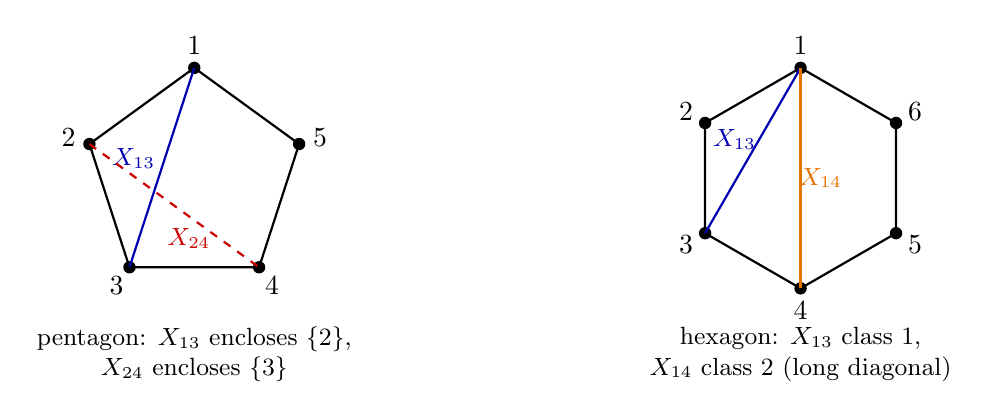
\begin{tikzpicture}[scale=1.4]

\foreach \i/\angle in {1/90, 2/162, 3/234, 4/306, 5/18}{
  \coordinate (P\i) at (\angle:1);
  \fill (P\i) circle (1.6pt);
  \node at (\angle:1.2) {$\i$};
}
\draw[thick] (P1) -- (P2) -- (P3) -- (P4) -- (P5) -- cycle;
\draw[blue!70!black, thick] (P1) -- (P3);
\node[blue!70!black, font=\small] at (-0.55, 0.18) {$X_{13}$};
\draw[red!80!black, thick, dashed] (P2) -- (P4);
\node[red!80!black, font=\small] at (-0.05, -0.55) {$X_{24}$};
\node[align=center, font=\small] at (0,-1.6) {pentagon: $X_{13}$ encloses $\{2\}$,\\ $X_{24}$ encloses $\{3\}$};

\begin{scope}[xshift=5.5cm]
\foreach \i/\angle in {1/90, 2/150, 3/210, 4/270, 5/330, 6/30}{
  \coordinate (Q\i) at (\angle:1);
  \fill (Q\i) circle (1.6pt);
  \node at (\angle:1.2) {$\i$};
}
\draw[thick] (Q1) -- (Q2) -- (Q3) -- (Q4) -- (Q5) -- (Q6) -- cycle;
\draw[blue!70!black, thick] (Q1) -- (Q3);
\node[blue!70!black, font=\small] at (-0.6, 0.35) {$X_{13}$};
\draw[orange!90!black, thick] (Q1) -- (Q4);
\node[orange!90!black, font=\small] at (0.18, 0.0) {$X_{14}$};
\node[align=center, font=\small] at (0,-1.6) {hexagon: $X_{13}$ class~1,\\ $X_{14}$ class~2 (long diagonal)};
\end{scope}
\end{tikzpicture}
\end{center}

\medskip
\noindent
The class is the right invariant for the kill mechanism: the algebraic ``layer'' at which the cyclic zero $Z_r$ kills a multiset $M$ matches the class of the substituted chord that fingerprints it. New chord class $\leftrightarrow$ new kill layer, both born together at $n = 2k+2$. We make this dictionary precise in \S\ref{sec:masterformula}.

A standard combinatorial fact will be used throughout, and it is the geometric reason the proof works:
\begin{lemma}[Crossing $=$ enclosed-vertex sweep] \label{lem:crossing}
Two chords $X_{ij}$ and $X_{rs}$ of a convex polygon cross in the interior if and only if exactly one endpoint of $X_{rs}$ lies in the enclosed arc of $X_{ij}$ (equivalently in $E(X_{ij})$), and the other lies in the outer arc.
\end{lemma}
\begin{proof}
Two chords of a convex polygon cross iff their four endpoints alternate around the boundary. Fix $X_{ij}$ and consider the two arcs it cuts off. The endpoints of $X_{rs}$ either both lie in the same arc (no alternation, no crossing) or one in each (alternation, crossing).
\end{proof}

\noindent
The consequence is the key geometric fact. Every \emph{non-local pair of chords} --- that is, every crossing pair --- has the form ``one chord with enclosed vertex $v$; another chord starting at $v$.'' The cyclic zeros, as we will see, are tailor-built to kill exactly such pairings, because each $Z_r$ has two substituted chords that begin at one specified vertex. The vertex is the enclosed vertex of the special chord at that zone.

\subsection{Feynman diagrams as triangulations} \label{sec:feyntri}

For color-ordered $\Tr(\phi^3)$ tree amplitudes, the Feynman expansion has a clean geometric image, established in Arkani-Hamed--Bai--He--Yan \cite{ABHY}: \emph{planar cubic Feynman diagrams are in bijection with triangulations of the $n$-gon}. A triangulation $T$ is a maximal set of non-crossing chords; it has $n-3$ elements and partitions the polygon into $n-2$ triangles. The bijection is the obvious one: each chord is a propagator $1/X_c$, each triangle is a cubic vertex. The number of triangulations is the Catalan number $C_{n-2}$. The tree amplitude is
\begin{equation}
A_n \;=\; \sum_{T\text{ triangulation}} \;\prod_{c\,\in\,T} \frac{1}{X_c}.
\label{eq:Antree}
\end{equation}

\begin{center}
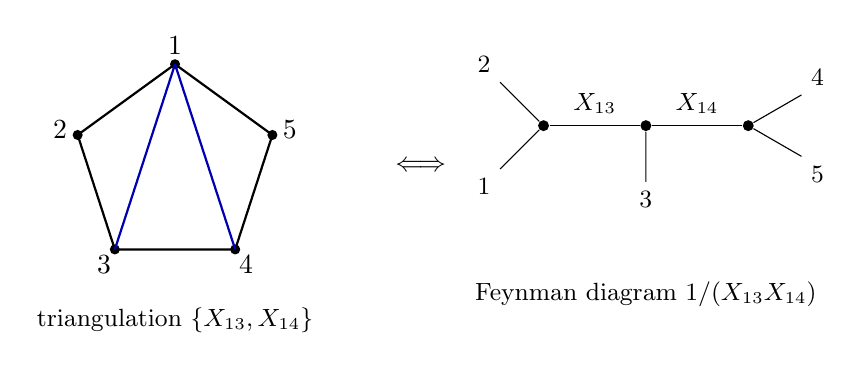
\begin{tikzpicture}[scale=1.3]

\foreach \i/\angle in {1/90, 2/162, 3/234, 4/306, 5/18}{
  \coordinate (P\i) at (\angle:1);
  \fill (P\i) circle (1.4pt);
  \node at (\angle:1.18) {$\i$};
}
\draw[thick] (P1) -- (P2) -- (P3) -- (P4) -- (P5) -- cycle;
\draw[blue!70!black, thick] (P1) -- (P3);
\draw[blue!70!black, thick] (P1) -- (P4);
\node at (0,-1.5) {\small triangulation $\{X_{13}, X_{14}\}$};

\begin{scope}[xshift=2.4cm, yshift=0cm]
\node at (0, 0) {$\Longleftrightarrow$};
\end{scope}

\begin{scope}[xshift=5.0cm]
\node[circle, fill, inner sep=1.4pt] (v1) at (-1.4, 0.4) {};
\node[circle, fill, inner sep=1.4pt] (v2) at (-0.4, 0.4) {};
\node[circle, fill, inner sep=1.4pt] (v3) at ( 0.6, 0.4) {};
% v1: two input legs (1, 2) coming in from the left (steeper to clear the iff arrow)
\draw (v1) -- ++(135:0.6) node[above left, font=\small] {$2$};
\draw (v1) -- ++(225:0.6) node[below left, font=\small] {$1$};
% propagator X_{13}
\draw (v1) -- (v2);
\node[above=1pt, font=\small] at ($(v1)!0.5!(v2)$) {$X_{13}$};
% v2: middle vertex with leg 3 going DOWN
\draw (v2) -- ++(270:0.55) node[below, font=\small] {$3$};
% propagator X_{14}
\draw (v2) -- (v3);
\node[above=1pt, font=\small] at ($(v2)!0.5!(v3)$) {$X_{14}$};
% v3: two output legs (4, 5) going out to the right
\draw (v3) -- ++( 30:0.6) node[above right, font=\small] {$4$};
\draw (v3) -- ++(-30:0.6) node[below right, font=\small] {$5$};
\node at (-0.4, -1.25) {\small Feynman diagram $1/(X_{13}X_{14})$};
\end{scope}

\end{tikzpicture}
\end{center}

\noindent
The pentagon has five triangulations and they are exactly the five Feynman diagrams of $A_5$.

For our purposes the important consequences are:

\begin{enumerate}
  \item[(L)] \textbf{Locality.} A monomial $1/(X_{a}X_{b}\cdots X_{n-3\text{ factors}})$ corresponds to a tree-level Feynman diagram if and only if its chords form a triangulation, i.e.\ are pairwise non-crossing.
  \item[(NL)] \textbf{Non-locality.} A monomial is non-local exactly when its chord multiset either contains a repeat (a chord appearing with multiplicity $\geq 2$) or contains a crossing pair. Both possibilities have a sharp geometric meaning: a repeat is a double pole on a single propagator, a crossing pair is two channels that mutually obstruct one another.
\end{enumerate}

\noindent
The general rational ansatz $B$ is a sum over \emph{all} multisets of size $n-3$, both local and non-local. The mission of the cyclic-zero conditions is to force every non-local coefficient to vanish, leaving exactly the $C_{n-2}$ triangulations.

\subsection{Hidden zeros and chord birth: the master formula} \label{sec:masterformula}

We now arrive at the heart of the geometric story. At each cyclic zero $Z_r$ --- defined by $c_{r,j}=0$ for all non-adjacent $j$ --- the linear constraints on the kinematic mesh have a single, vertex-local solution. Apply Rodina's mesh identity
\[
c_{i,j} = X_{i,j+1} + X_{i+1,j} - X_{i,j} - X_{i+1,j+1}
\]
to each constraint and unfold; what comes out is one universal substitution rule:

\begin{equation}
\boxed{
\quad X_{r+1,\,j} \;=\; X_{r,j} \;-\; X_{r,r+2} \qquad \text{for all admissible $j$.}\quad
}
\label{eq:masterformula}
\end{equation}

This is the master formula. It generates every $Z_r$-substitution at every $n$, with no special cases. The bare case is automatic: when $j = r-1$, the right-hand side $X_{r,r-1}$ is an adjacent leg, hence zero, and the substitution becomes $X_{r+1,r-1} = -X_{r,r+2}$. There is nothing more to memorize.

The geometric reading is what we want to bring out. Imagine that we have just inserted a new vertex $r+1$ between $r$ and $r+2$ on the boundary. The chord $X_{r,r+2}$, which used to be a leg, is now a chord --- it is the \emph{special chord} of the zone, denoted $X_*$. The vertex $r+1$ is its enclosed vertex. Every chord $X_{r+1,j}$ that starts at the new vertex is \emph{born} as a linear combination of two older chords:
\[
\underbrace{X_{r+1,j}}_{\text{newborn}} \;=\; \underbrace{X_{r,j}}_{\text{older sibling, the \emph{companion}}} \;-\; \underbrace{X_{r,r+2}}_{\text{the special chord }X_*}.
\]
This is the chord-birth picture. There are exactly $n-3$ newborns, one for each admissible $j \in \{r+3, r+4, \dots, r-1\}$. Among them:

\begin{itemize}
  \item One is born \emph{bare}: the case $j = r-1$ has companion $X_{r,r-1}=0$, giving $X_{r+1,r-1} = -X_*$. There is no genuine free chord on the right; this newborn is a multiple of $X_*$ and contributes only the leading Laurent order.
  \item The other $n-4$ are born \emph{constrained}: each has a companion $X_{r,j} \in F_r$ that survives in the free set and links the newborn to it via the hidden-zero relation.
\end{itemize}

The chord $X_{r,r+2} = X_*$ is the propagator at this step. It appears on the right-hand side of every birth equation. Every Laurent expansion at $Z_r$ is in $1/X_*$:
\[
\frac{1}{X_{r+1,j}} \;=\; \frac{1}{X_{r,j} - X_*} \;=\; -\frac{1}{X_*} - \frac{X_{r,j}}{X_*^2} - \frac{X_{r,j}^2}{X_*^3} - \cdots ,
\]
so $X_*$ controls the kill structure entirely. Once a chord is identified with $X_*$, it never leaves the right-hand side: it is the propagator that does the work for this particular cyclic zero, and its contribution is fixed at all subsequent orders. This is what we mean when we say ``$X_{1,n}$ becomes a propagator at every step'' for the canonical zone $Z_n$ where $X_* = X_{1,n}$. By cyclic relabeling, every short diagonal $X_{r,r+2}$ takes its turn.

The classification of newborns into ``free'' versus ``constrained'' has a direct combinatorial counterpart: which of the $n-3$ chord births contribute companions in the free set $F_r$. Each constrained birth gives one such companion, and the resulting set of $n-4$ companions is exactly the data needed for the local kill-test (\S3).

\medskip

\begin{center}
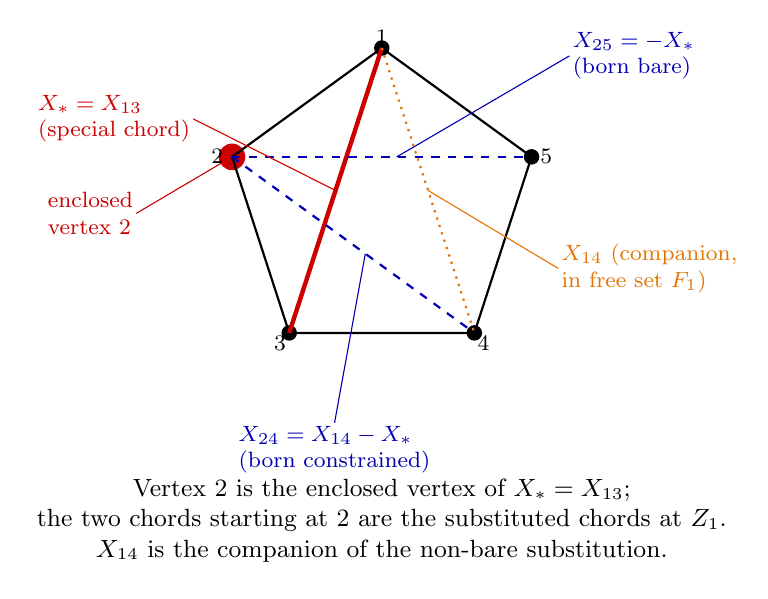
\begin{tikzpicture}[scale=2.0,
    label/.style={font=\footnotesize, inner sep=1pt}]

% Pentagon vertices
\foreach \i/\angle in {1/90, 2/162, 3/234, 4/306, 5/18}{
  \coordinate (P\i) at (\angle:1);
}
\fill (P1) circle (1.4pt);
\fill (P3) circle (1.4pt);
\fill (P4) circle (1.4pt);
\fill (P5) circle (1.4pt);
\fill[red!80!black] (P2) circle (2.4pt);

\node[label, above]      at (P1) {$1$};
\node[label, left=2pt]   at (P2) {$2$};
\node[label, below left] at (P3) {$3$};
\node[label, below right]at (P4) {$4$};
\node[label, right=2pt]  at (P5) {$5$};

% Polygon boundary
\draw[thick] (P1) -- (P2) -- (P3) -- (P4) -- (P5) -- cycle;

% Special chord (red, thick)
\draw[red!80!black, ultra thick] (P1) -- (P3);

% Substituted chords (blue, dashed)
\draw[blue!70!black, thick, dashed] (P2) -- (P4);
\draw[blue!70!black, thick, dashed] (P2) -- (P5);

% Companion (orange, dotted) — free chord
\draw[orange!90!black, thick, dotted] (P1) -- (P4);

% External labels with leader lines
% Special X*
\node[label, red!80!black, align=left] (Lstar) at (-1.7, 0.55) {$X_* = X_{13}$\\ (special chord)};
\draw[red!80!black, thin] (Lstar.east) -- ($(P1)!0.5!(P3)$);

% Enclosed vertex
\node[label, red!80!black, align=left] (Lenc) at (-1.85, -0.05) {enclosed\\ vertex $2$};
\draw[red!80!black, thin] (Lenc.east) -- (P2);

% X_24 (non-bare)
\node[label, blue!70!black, align=left] (LX24) at (-0.3, -1.55) {$X_{24} = X_{14} - X_*$\\ (born constrained)};
\draw[blue!70!black, thin] (LX24.north) -- ($(P2)!0.55!(P4)$);

% X_25 (bare)
\node[label, blue!70!black, align=left] (LX25) at (1.6, 0.95) {$X_{25} = -X_*$\\ (born bare)};
\draw[blue!70!black, thin] (LX25.west) -- ($(P2)!0.55!(P5)$);

% Companion X_14
\node[label, orange!90!black, align=left] (LX14) at (1.7, -0.4) {$X_{14}$ (companion,\\ in free set $F_1$)};
\draw[orange!90!black, thin] (LX14.west) -- ($(P1)!0.5!(P4)$);

\node[align=center, font=\small] at (0, -2.0)
{Vertex 2 is the enclosed vertex of $X_*=X_{13}$;\\
the two chords starting at 2 are the substituted chords at $Z_1$.\\
$X_{14}$ is the companion of the non-bare substitution.};

\end{tikzpicture}
\end{center}

\medskip
\noindent
This is the full content of $Z_1$ at $n=5$. Read it geometrically: the special chord $X_*=X_{13}$ encloses vertex 2; the two chords that begin at vertex 2 (namely $X_{24}, X_{25}$) are the ones forced into substitution; the remaining chords ($X_{14}, X_{35}$) are the free set. Cycling $r \mapsto r+1$ rotates this picture around the polygon and gives all five zones. At higher $n$ the picture is identical, just with more chords born at each step.

\subsection*{Born free, born constrained: the algebraic-geometric dictionary}

Putting everything from this subsection in one place:

\begin{center}
\begin{tabular}{l|l}
\textbf{Geometric data at $Z_r$} & \textbf{Algebraic role} \\\hline
Special chord $X_*=X_{r,r+2}$ & Laurent variable; the propagator at this step \\
Enclosed vertex $r+1 \in E(X_*)$ & Vertex from which all substituted chords originate \\
Chords starting at $r+1$ & Substituted chords (newborns) \\
\quad those with companion $\in F_r$ & ``Born constrained'' --- $n-4$ of these \\
\quad the bare one (companion $=0$) & ``Born free of a companion'' --- 1 of these \\
Other planar chords & Free set $F_r$ ($\big|F_r\big| = \binom{n}{2}-n-(n-3)-1$)
\end{tabular}
\end{center}

\noindent
Every cyclic zero is one snapshot of this same picture, rotated. The sum over zones $r=1,\dots,n$ sweeps every short diagonal through the role of $X_*$, every vertex through the role of the enclosed vertex, and every crossing pair gets isolated by at least one zone.

\subsection{Why locality has to hold: closed loops and acausality} \label{sec:closedloop}

The proof sections that follow show \emph{algebraically} that the cyclic zeros kill every non-local coefficient. We close this section with a physical argument for why one should expect this on causal grounds. The argument has four parts; we walk through each in turn.

\subsubsection*{Part 1: closed timelike curves require $v > c$}

In special relativity, a worldline on a $(t,x)$ Minkowski diagram is a curve whose tangent vector $(\dot t, \dot x)$ has $\dot t \geq 0$ (we follow proper time forward) and $|\dot x / \dot t| \leq c$ (subluminal). Plotting time vertically and space horizontally:

\begin{center}
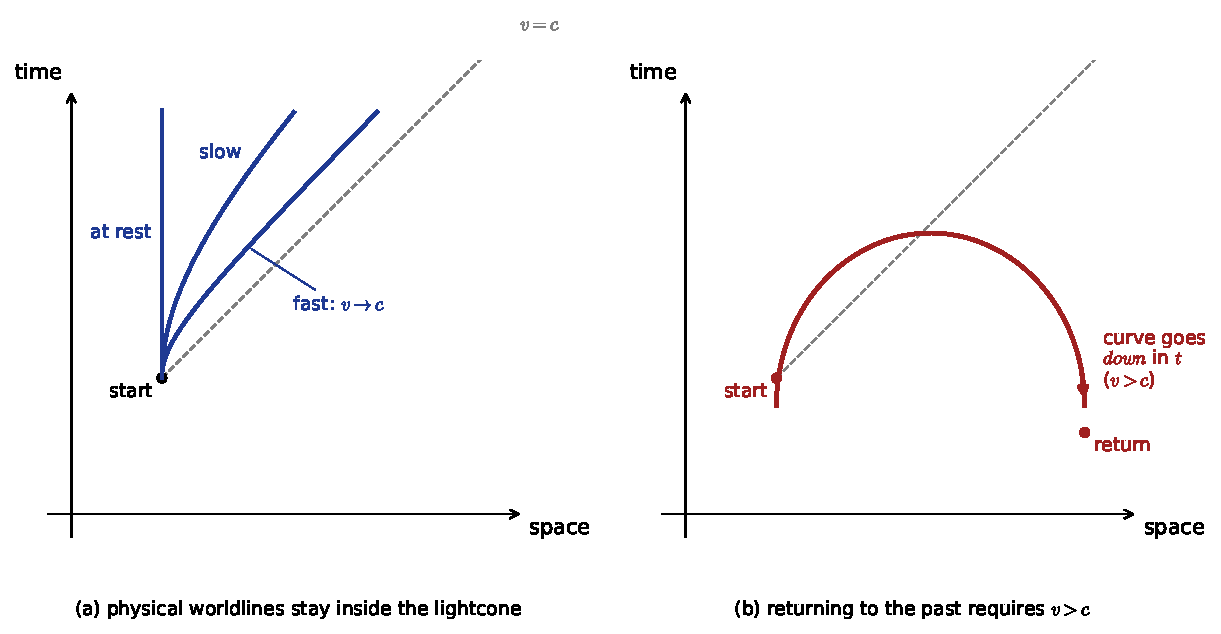
\includegraphics[width=0.95\textwidth]{figures/worldline_figure.pdf}
\end{center}

\noindent
On (a), allowed worldlines all sit on the timelike side of the lightcone; as speed grows the curve tilts toward $45^\circ$, and at $v = c$ it becomes the lightcone itself. To \emph{return} to a previous spacetime point --- to close the loop --- the worldline must at some segment tilt past horizontal, as in (b): the tangent $(\dot t, \dot x)$ acquires $\dot t < 0$, meaning the particle is moving backward in time, which by the relativistic dispersion relation requires $|\dot x / \dot t| > c$.

So: \emph{closed timelike curves $\Leftrightarrow$ travel to the past $\Leftrightarrow$ velocity $> c$.}

\subsubsection*{Part 2: Feynman diagrams are time-oriented}

A trivalent vertex in a tree-level Feynman diagram has a definite past/future structure inherited from the underlying field theory: two legs come in from the past, one leg goes out toward the future (an interaction), or one leg comes in and two legs go out toward the future (particle production). Drawing the diagram with time pointing upward, every internal propagator is a time-oriented edge.

\begin{center}
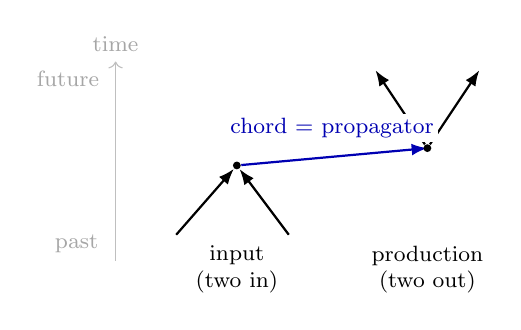
\begin{tikzpicture}[scale=1.1,
    every node/.style={font=\small},
    timeArrow/.style={-{Latex[length=2.0mm]}, thick}]

% Vertical time axis
\draw[->, gray!50] (-2.0, -0.6) -- (-2.0, 1.7) node[above, gray!70, font=\footnotesize] {time};
\node[gray!70, font=\footnotesize] at (-2.45, -0.4) {past};
\node[gray!70, font=\footnotesize] at (-2.55, 1.5) {future};

% A 2-into-1 vertex (input/interaction)
\node[circle, fill, inner sep=1.0pt] (vIn) at (-0.6, 0.5) {};
\draw[timeArrow] (-1.3, -0.3) -- (vIn);
\draw[timeArrow] ( 0.0, -0.3) -- (vIn);
\draw[timeArrow, blue!70!black] (vIn) -- (1.6, 0.7);
\node[font=\footnotesize, align=center] at (-0.6, -0.7) {input\\ (two in)};

% Vertex 2 (production)
\node[circle, fill, inner sep=1.0pt] (vOut) at (1.6, 0.7) {};
\draw[timeArrow] (vOut) -- (1.0, 1.6);
\draw[timeArrow] (vOut) -- (2.2, 1.6);
\node[font=\footnotesize, align=center] at (1.6, -0.7) {production\\ (two out)};

\path (vIn) -- (vOut) node[midway, above=5pt, blue!70!black, font=\footnotesize, fill=white, inner sep=1.5pt] {chord = propagator};

\end{tikzpicture}
\end{center}

\noindent
The blue propagator is the realization, in the Feynman picture, of a chord of the polygon: it is an internal edge connecting two interaction vertices, with a definite direction of time-flow.

\subsubsection*{Part 3: Triangulation $\leftrightarrow$ Feynman, in pictures}

We saw the duality in \S\ref{sec:feyntri} for the pentagon. Here are the two smallest cases drawn in the same style as the four-part argument:

\begin{center}
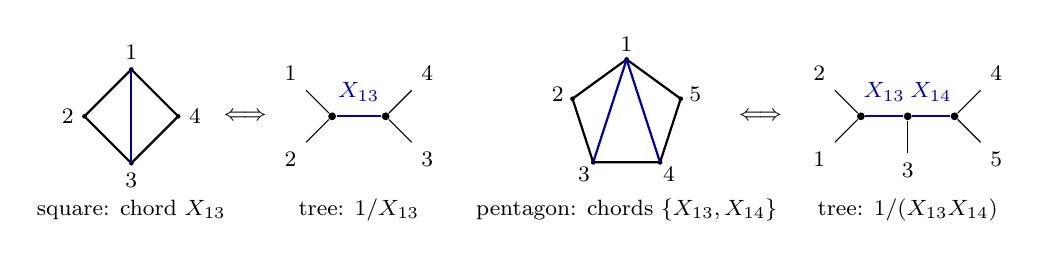
\begin{tikzpicture}[scale=0.85, every node/.style={font=\footnotesize}]

% =================== n = 4 case ===================

% Square — axis-aligned: 1 top, 2 left, 3 bottom, 4 right (CCW)
\begin{scope}
\foreach \i/\ang in {1/90, 2/180, 3/270, 4/0}{
  \coordinate (S\i) at (\ang:0.7);
  \fill (S\i) circle (1.0pt);
  \node at (\ang:0.95) {$\i$};
}
\draw[thick] (S1) -- (S2) -- (S3) -- (S4) -- cycle;
\draw[blue!70!black, thick] (S1) -- (S3);
\node at (0, -1.4) {square: chord $X_{13}$};
\end{scope}

\node at (1.7, 0) {$\Longleftrightarrow$};

% Feynman tree for n=4
\begin{scope}[xshift=3.4cm]
\node[circle, fill, inner sep=1.0pt] (a) at (-0.4, 0) {};
\node[circle, fill, inner sep=1.0pt] (b) at ( 0.4, 0) {};
% LEFT vertex: legs 1 (up-left), 2 (down-left)
\draw (a) -- ++(135:0.55) node[above left] {$1$};
\draw (a) -- ++(225:0.55) node[below left] {$2$};
% RIGHT vertex: legs 4 (up-right), 3 (down-right)
\draw (b) -- ++( 45:0.55) node[above right] {$4$};
\draw (b) -- ++(-45:0.55) node[below right] {$3$};
% propagator
\draw[blue!70!black, thick] (a) -- (b);
\node[blue!70!black, above=2pt, font=\footnotesize] at (0, 0) {$X_{13}$};
\node at (0, -1.4) {tree: $1/X_{13}$};
\end{scope}

% =================== n = 5 case ===================

% Pentagon — same layout as §2.2 (1 top, 2 upper-left, 3 lower-left, 4 lower-right, 5 upper-right)
\begin{scope}[xshift=7.4cm]
\foreach \i/\ang in {1/90, 2/162, 3/234, 4/306, 5/18}{
  \coordinate (Q\i) at (\ang:0.85);
  \fill (Q\i) circle (1.0pt);
  \node at (\ang:1.08) {$\i$};
}
\draw[thick] (Q1) -- (Q2) -- (Q3) -- (Q4) -- (Q5) -- cycle;
\draw[blue!70!black, thick] (Q1) -- (Q3);
\draw[blue!70!black, thick] (Q1) -- (Q4);
\node at (0, -1.4) {pentagon: chords $\{X_{13},X_{14}\}$};
\end{scope}

\node at (9.4, 0) {$\Longleftrightarrow$};

% Feynman tree for n=5 — matches §2.2 layout (leg 3 going DOWN; 1,2 left inputs; 4,5 right outputs)
\begin{scope}[xshift=11.6cm]
\node[circle, fill, inner sep=1.0pt] (u1) at (-0.7, 0) {};
\node[circle, fill, inner sep=1.0pt] (u2) at ( 0.0, 0) {};
\node[circle, fill, inner sep=1.0pt] (u3) at ( 0.7, 0) {};
% u1: input legs 2 (up-left) and 1 (down-left)
\draw (u1) -- ++(135:0.55) node[above left] {$2$};
\draw (u1) -- ++(225:0.55) node[below left] {$1$};
% u2: middle vertex, leg 3 going DOWN
\draw (u2) -- ++(270:0.55) node[below] {$3$};
% u3: output legs 4 (up-right), 5 (down-right)
\draw (u3) -- ++( 45:0.55) node[above right] {$4$};
\draw (u3) -- ++(-45:0.55) node[below right] {$5$};
\draw[blue!70!black, thick] (u1) -- (u2);
\node[blue!70!black, above=2pt, font=\footnotesize] at ($(u1)!0.5!(u2)$) {$X_{13}$};
\draw[blue!70!black, thick] (u2) -- (u3);
\node[blue!70!black, above=2pt, font=\footnotesize] at ($(u2)!0.5!(u3)$) {$X_{14}$};
\node at (0, -1.4) {tree: $1/(X_{13}X_{14})$};
\end{scope}

\end{tikzpicture}
\end{center}

\noindent
In each case, every triangle of the (non-crossing) triangulation is a trivalent vertex, every chord is a propagator, and every external edge is a leg. The diagram has a consistent time-flow once we choose a direction across the polygon.

\subsubsection*{Part 4: an intersection forces a closed Feynman loop}

Now apply the construction of Part 3 to a polygon with two \emph{intersecting} chords. Take the pentagon with chords $\{X_{13}, X_{24}\}$:

\begin{center}
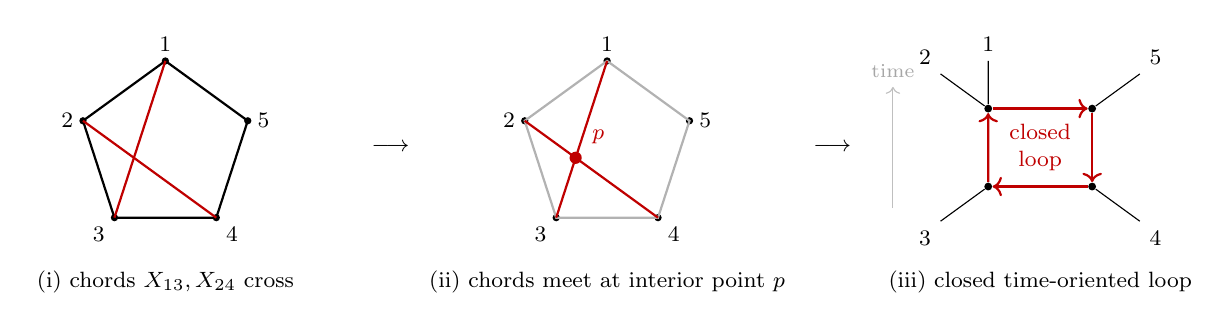
\begin{tikzpicture}[scale=1.1, every node/.style={font=\footnotesize}]

% Step (i): pentagon with crossing
\begin{scope}
\foreach \i/\ang in {1/90, 2/162, 3/234, 4/306, 5/18}{
  \coordinate (P\i) at (\ang:1);
  \fill (P\i) circle (1.2pt);
}
\node[above]      at (P1) {$1$};
\node[left]       at (P2) {$2$};
\node[below left] at (P3) {$3$};
\node[below right]at (P4) {$4$};
\node[right]      at (P5) {$5$};
\draw[thick] (P1) -- (P2) -- (P3) -- (P4) -- (P5) -- cycle;
\draw[red!75!black, thick] (P1) -- (P3);
\draw[red!75!black, thick] (P2) -- (P4);
\node at (0, -1.55) {(i) chords $X_{13}, X_{24}$ cross};
\end{scope}

\node at (2.6, 0) {$\longrightarrow$};

% Step (ii): mark the intersection as a phantom vertex
\begin{scope}[xshift=5.1cm]
\foreach \i/\ang in {1/90, 2/162, 3/234, 4/306, 5/18}{
  \coordinate (R\i) at (\ang:1);
  \fill (R\i) circle (1.2pt);
}
\node[above]      at (R1) {$1$};
\node[left]       at (R2) {$2$};
\node[below left] at (R3) {$3$};
\node[below right]at (R4) {$4$};
\node[right]      at (R5) {$5$};
\draw[thick, gray!60] (R1) -- (R2) -- (R3) -- (R4) -- (R5) -- cycle;
\draw[red!75!black, thick] (R1) -- (R3);
\draw[red!75!black, thick] (R2) -- (R4);
% Mark the intersection point as p
\coordinate (I) at (intersection of R1--R3 and R2--R4);
\fill[red!75!black] (I) circle (2pt);
\node[red!75!black, font=\footnotesize, anchor=south west] at ($(I) + (0.08, 0.05)$) {$p$};
\node at (0, -1.55) {(ii) chords meet at interior point $p$};
\end{scope}

\node at (7.7, 0) {$\longrightarrow$};

% Step (iii): closed Feynman loop
\begin{scope}[xshift=10.1cm]
\node[circle, fill, inner sep=1.0pt] (w1) at (-0.6,  0.45) {};
\node[circle, fill, inner sep=1.0pt] (w2) at ( 0.6,  0.45) {};
\node[circle, fill, inner sep=1.0pt] (w3) at ( 0.6, -0.45) {};
\node[circle, fill, inner sep=1.0pt] (w4) at (-0.6, -0.45) {};
% External legs
\draw (w1) -- ++(-0.55,  0.4) node[above left] {$2$};
\draw (w1) -- ++( 0.0,  0.55) node[above] {$1$};
\draw (w2) -- ++( 0.55,  0.4) node[above right] {$5$};
\draw (w3) -- ++( 0.55, -0.4) node[below right] {$4$};
\draw (w4) -- ++(-0.55, -0.4) node[below left] {$3$};
% Closed loop with arrows
\draw[red!75!black, thick, ->] (w4) -- (w1);
\draw[red!75!black, thick, ->] (w1) -- (w2);
\draw[red!75!black, thick, ->] (w2) -- (w3);
\draw[red!75!black, thick, ->] (w3) -- (w4);
% Time arrow
\draw[->, gray!50] (-1.7, -0.7) -- (-1.7, 0.7) node[above, gray!70, font=\scriptsize] {time};
\node[red!75!black, font=\footnotesize, align=center] at (0, 0) {closed\\ loop};
\node at (0, -1.55) {(iii) closed time-oriented loop};
\end{scope}

\end{tikzpicture}
\end{center}

\noindent
Here is what happens. A non-crossing triangulation has $n-3$ chords meeting only at polygon vertices, giving a tree (no internal loops). When two chords cross, they create an interior intersection point $p$ that is not a polygon vertex. If we still try to apply the rule of Part~3 ``each chord is a propagator,'' we must treat $p$ as a \emph{phantom vertex} --- a heuristic interaction point with no underlying field-theory vertex --- and the four chord-pieces meeting at $p$ generate a closed circuit in the Feynman graph: starting at one chord-endpoint, we travel along $X_{13}$, turn at $p$, travel along $X_{24}$, turn at the next polygon vertex, and so on, until we return to the starting endpoint.

By Part~2, every propagator in this circuit is time-oriented. Following the time-arrows around the closed loop, the loop must rise (toward the future) along some propagators and descend (toward the past) along others, since it returns to its starting point. The descending propagators are exactly the case from Part~1: a worldline whose tangent has $\dot t < 0$, which requires $v > c$.

\paragraph{The conclusion.}
A pair of crossing chords corresponds to a Feynman channel that, interpreted as a process in spacetime, contains a closed time-oriented circuit. By Part~1 such a circuit requires superluminal propagation, hence violates causality. The cyclic hidden zeros, by killing every non-local (= crossing or repeated) coefficient, are forbidding exactly the channels that would correspond to acausal processes.

Locality, in this picture, is the absence of acausal Feynman channels --- equivalently, the requirement that the amplitude support only chord systems that can be drawn as planar trees, i.e.\ triangulations.

\paragraph{Where rigor stops.}
The argument above is geometric and physical, not a theorem in the strict sense of the rest of the paper. Two places where it would need to be tightened:

\begin{itemize}
  \item \emph{Phantom vertices.} The interior intersection of two chords is not, in any standard formulation of color-ordered $\Tr(\phi^3)$, a genuine interaction vertex. Reading the crossing as ``a vertex'' is a heuristic; the precise statement is that no planar Feynman graph for the cyclic ordering can realize $1/(X_{ij}X_{rs})$ when the two chords cross, and the reason is the closed-loop obstruction sketched above.
  \item \emph{Time direction across the polygon.} ``Time-flow across the polygon'' depends on a choice of direction; different choices give different traversals of the closed loop, but the same conclusion (some segment of the loop must descend in time). A clean formal statement would use the worldline path-integral picture, where each chord is the worldline of a virtual particle and the no-closed-timelike-curve condition is intrinsic.
\end{itemize}

\noindent
The author has a draft of the worldline picture in the companion note on flat connections \cite{flatconn}. The closed-loop / acausality argument should be understood as the physical motivation for why the algebraic kill mechanism in the next sections \emph{has} to give what it does: any other answer would correspond to an amplitude that supports superluminal channels.

\subsection*{Forward}

The remainder of the paper turns the chord-birth picture above into an explicit kill mechanism. \S\ref{sec:masterformula} already contains the master formula; \S3 promotes it to a local kill-test that decides, for each non-local multiset $M$ and each cyclic zone $Z_r$, whether $M$ is killed at that zone and at which Laurent layer. \S4 verifies the kill-test by hand at $n=5$, where the polygon has only class-1 chords and the picture is two-dimensional. \S5 carries it out at $n=6$, where the appearance of class-2 (long-diagonal) chords introduces a new layer of kills, exactly as the class--layer dictionary predicts. \S6 reduces the general-$n$ theorem to a single combinatorial blocking-set lemma about polygon multisets, and reports the numerical verification of that lemma at $n = 7$. The flat-connection physics of \S\ref{sec:closedloop} is offered for motivation; the proof itself is self-contained at the level of polynomial identities and never invokes worldlines.

\begin{thebibliography}{99}
\bibitem{ABHY} N. Arkani-Hamed, Y.~Bai, S.~He, G.~Yan, ``Scattering Forms and the Positive Geometry of Kinematics, Color and the Worldsheet,'' \emph{JHEP} \textbf{05} (2018) 096; arXiv:1711.09102.
\bibitem{Rodina} G.~Rodina, ``Hidden zeros are equivalent to enhanced ultraviolet scaling and lead to unique amplitudes in $\Tr(\phi^3)$ theory,'' arXiv:2406.04234.
\bibitem{ArkaniHamedHiddenZeros} N.~Arkani-Hamed et al., ``Hidden zeros for particle/string amplitudes and the unity of colored scalars, pions, and gluons,'' arXiv:2312.16282.
\bibitem{flatconn} J.~[Author], ``Flat Connections and the Emergence of Unitarity and Locality,'' draft, 2026.
\end{thebibliography}

\end{document}
